% To compile run lualatex and bibtex (fontspec requires LuaLaTeX or XeLaTeX)
%   lualatex paper -> bibtex paper -> lualatex paper -> lualatex paper
%
% =====================================================================
% Enabling Automated Controller Deployment in IoT-Enabled Building Systems with GraphRAG
% Target: 2026 European Conference on Computing in Construction (EC3), 8 pages, two-column.
% Adapted from paper/paper.tex to the official EC3_2026 template.
% Citation style: Harvard author-date via natbib, apalikenonitalic.bst
% =====================================================================

%%%%%%%%%%%%%%%%%%%%%%%%%%%%%%%%%%%%%%%%%%%%%%%%%%%%%%%%%%%%%%%%%%%%%%%%%%%%%%%%%%%%%
% EC3 Latex template
%%%%%%%%%%%%%%%%%%%%%%%%%%%%%%%%%%%%%%%%%%%%%%%%%%%%%%%%%%%%%%%%%%%%%%%%%%%
% TODO change to double column
\documentclass[twocolumn, 10pt, A4paper]{article}

\usepackage{fontspec}
\setmainfont[
  UprightFont    = {Times New Roman},
  ItalicFont     = {Times New Roman Italic},
  BoldFont       = {Times New Roman Bold},
  BoldItalicFont = {Times New Roman Bold Italic}
]{Times New Roman}
% Commented out because of above
% http://tug.ctan.org/tex-archive/macros/latex/contrib/geometry/
\usepackage{geometry}
\geometry{ a4paper, total={170mm,257mm}, top=25mm, left=20mm, }

\usepackage{amssymb}
\usepackage{newtxmath} % optional, for math
\usepackage[justification=centering]{caption}

\usepackage{enumitem}% To reduce separation between bullets or itemized lists
% Use with [noitemsep]EC3_2026

\usepackage{natbib}

\usepackage{amsmath}
\usepackage{epsfig}
\usepackage{graphicx}
\usepackage{vmargin}
\usepackage{url}
\usepackage{tabularx}
\usepackage{boxedminipage}
\usepackage{booktabs}% rules used by the manuscript tables

\usepackage{newtxtext}%This package is needed for bold and Italic fonts.

\usepackage{lastpage} % for the number of the last page in the document
\usepackage{fancyhdr}
\usepackage{soul} % for defining underline thickness

% -------------------------------------------------------------------
% Different font in captions
\newcommand{\captionfonts}{\fontsize{9}{9}\it}
\setlength{\abovecaptionskip}{-3pt} %% That it used for look like Word
\setlength{\belowcaptionskip}{0pt}

\makeatletter  % Allow the use of @ in command names
\long\def\@makecaption#1#2{ %
  \vskip\abovecaptionskip
  \sbox\@tempboxa{{\captionfonts #1: #2}}%
   \ifdim \wd\@tempboxa >\hsize
	{\centering\captionfonts #1: #2\par}
   \else
    \hbox to\hsize{\hfil\box\@tempboxa\hfil}%
   \fi
  \vskip\belowcaptionskip}
\makeatother   % Cancel the effect of \makeatletter
% -------------------------------------------------------------------

% Fuzz -------------------------------------------------------------------
\hfuzz4pt % Don't bother to report over-full boxes if over-edge is < 2pt
\vfuzz=\hfuzz

% Line spacing -----------------------------------------------------------
\newlength{\defbaselineskip}
\setlength{\defbaselineskip}{\baselineskip}
\newcommand{\setlinespacing}[1]%
           {\setlength{\baselineskip}{#1 \defbaselineskip}}
\newcommand{\doublespacing}{\setlength{\baselineskip}
                           {2.0 \defbaselineskip}}
\newcommand{\singlespacing}{\setlength{\baselineskip}{\defbaselineskip}}
\newcommand{\onehalfspacing}{\setlength{\baselineskip}
                           {1.5 \defbaselineskip}}

\hyphenation{TRNSYS}

% Page layout ------------------------------------------------------------
\setlength{\topmargin}{0mm}%
\setlength{\headheight}{25mm}
\setlength{\headsep}{0mm}
\setlength{\textwidth}{17cm}
\setlength{\textheight}{241mm}
\setlength{\hoffset}{-40.5mm}
\setlength{\footskip}{12pt}
\setlength{\parindent}{5mm}% EC3 guide: first paragraph line indented 5 mm
\setlength{\columnsep}{8mm}
\setcounter{secnumdepth}{-2} % headings are not numbered

% Additional design for tables ------------------------------------------
\makeatletter
\newsavebox\saved@arstrutbox
\newcommand*{\setarstrut}[1]{%
	\noalign{%
		\begingroup
		\global\setbox\saved@arstrutbox\copy\@arstrutbox
		\global\setbox\@arstrutbox\hbox{%
			\vrule \@height #1
			\@depth  0cm
			\@width\z@
		}%
		\endgroup
	}%
}
\newcommand*{\restorearstrut}{%
	\noalign{%
		\global\setbox\@arstrutbox\copy\saved@arstrutbox
	}%
}
\makeatother
\newcommand{\paddingtop}[2]{\setarstrut{#1} #2 \\ \restorearstrut}

%% Spacing between columns within the table
\setlength{\tabcolsep}{5mm}

% Spacing between text and formula -------------------------------------
\setlength{\abovedisplayshortskip}{3pt}
\setlength{\abovedisplayskip}{3pt}
\setlength{\belowdisplayskip}{3pt}
\setlength{\belowdisplayshortskip}{3pt}

% Set fonts for title, section and subsection headings -----------------
\makeatletter
\renewcommand\section{\@startsection{section}{1}{\z@}{6pt}{3pt}{\normalfont\large\bfseries}}
\renewcommand\subsection{\@startsection{subsection}{1}{\z@}{6pt}{3pt}{\normalfont\normalsize\bfseries}}
\renewcommand\subsubsection{\@startsection{subsubsection}{1}{\z@}{6pt}{3pt}{\normalfont\normalsize\itshape}}
\makeatother

\renewcommand\refname{}

\newcommand{\authorfont}{\fontsize{11}{14}\selectfont}
\newcommand{\titlefont}{\fontsize{12}{14}\selectfont \bf}
\newcommand{\headerfont}{\fontsize{10}{11}\selectfont}
\newcommand{\smallsmall}{\fontsize{3}{3}\selectfont}
\newcommand{\tablefont}{\fontsize{9}{9}\selectfont}

% -------------------------------------------------------------------------

\pagestyle{empty}

\bibliographystyle{apalikenonitalic}% needs apalikenonitalic.bst in workdir

% Contents ----------------------------------------------------------------
\begin{document}

\fancypagestyle{empty}{
  \vspace{5pt}
  \fancyhf{}% Clear header/footer
  \renewcommand{\headrulewidth}{2.25pt}
  \renewcommand{\headsep}{13pt}

  % Left logo: bottom aligned, flush left, no inner padding
  \fancyhead[L]{%
    \begin{tabular}[b]{@{}l@{}}
%      \includegraphics[height=1.8cm, trim={0 0.1cm 0 0}, clip]{img/LogoJPG.JPG}
      
\includegraphics[height=1.8cm]{img/2027ec3}
    \end{tabular}
  }

  % Center text: bottom aligned, centered
  % TODO
%  \fancyhead[C]{%
%    \begin{tabular}[b]{c}
%      2026 European Conference on Computing in Construction \\
%      Corfu, Greece \\
%      July 12--15, 2026
%    \end{tabular}
%  }

  % Right logo: bottom aligned, flush right, no inner padding
  \fancyhead[R]{%
    \begin{tabular}[b]{@{}r@{}}
      
\includegraphics[height=1.45cm, trim={0 0.1cm 0 0}, clip]{img/EC3_LOGO_2.png}
    \end{tabular}
  }
}

\date{}
\title{\vspace{-9mm} \titlefont Enabling Automated Controller Deployment in IoT-Enabled Building Systems with GraphRAG \vspace{-5.5mm}}
\author{
%\authorfont{Junsong Du$^1$, Rita Streblow$^1$, and Dirk Müller$^2$}\\
%\authorfont{$^1$RWTH Aachen University, Aachen, Germany}\\
%\authorfont{\texttt{junsong.du@eonerc.rwth-aachen.de}}\\
\authorfont{~}\\
\authorfont{~}\\
\vspace{-15mm}
}
\maketitle
\thispagestyle{empty}

% --------------------------------------------------------
\setul{2pt}{0.25pt}
\section*{Abstract}

Internet of Things (IoT) platforms are increasingly used to enhance building systems with real-time data and interaction capabilities.
However, the heterogeneity of existing IoT platforms and underlying building systems forces applications like demand-based HVAC control to be re-engineered for each deployment, which is commonly referred to as the cross-platform interoperability problem.
This paper presents a GraphRAG pipeline that automates controller deployment in IoT-enabled building systems using generated knowledge graphs (KGs).
The pipeline prompts a large language model (LLM) to retrieve deployment-relevant context from the graph and to generate a detailed controller configuration for a given target space for a specific IoT platform.
We validate the pipeline on two distinct IoT platforms, FIWARE and ioBroker, and compare it against two full-context LLM baselines supplied with raw metadata and with full KGs respectively.
Deployment accuracy is measured as precision and recall against expert-authored ground truth.
Results show that the GraphRAG pipeline outperforms both baselines, and it also enables local mid-size models (the Gemma4 family) to match the performance of a larger model (Gemini).

\vspace{0.5em}
\noindent\textbf{Keywords:} GraphRAG; knowledge graph; building automation; IoT platforms; large language models

% =====================================================================
\section{Introduction}
\label{sec:introduction}
% TODO this section is generated. Must be critically reviewed
%Room-level controller deployment in IoT-enabled buildings is a configuration problem before it is a hardware problem. Once sensors, actuators, and gateways are physically installed, the remaining effort is cognitive and clerical: an engineer reads the available points, decides which control strategy they can support, and encodes that decision into the data-interface syntax of the target platform. Commissioning is a sizeable recurring expense in building projects. \citet{crowe2020building}, analysing outcomes across 1,500 North American buildings, report median commissioning costs (2020 US dollars) of USD 2.85/m$^2$ for existing buildings and USD 8.78/m$^2$ for new construction, alongside energy savings that justify the expenditure. The cost sits largely in the labour of mapping intent to concrete device and point configurations, not in the devices themselves.
%
%That labour scales with heterogeneity. A building may expose its data through a standards-oriented middleware such as FIWARE, whose NGSI-LD information model is designed for cross-domain interoperability \citep{bauer2022fiware}, or through a lightweight, vendor-neutral automation platform of the class that \citet{setz2021comparison} review, to which ioBroker belongs. The two ecosystems describe comparable physical reality with incompatible object models, naming conventions, and interface syntax. The consequence is that configuration logic rarely ports between platforms, and reuse is blocked at the point where it would save the most effort. \citet{fierro2020shepherding} show that even within a single building's lifecycle the digital representations (gbXML, BuildingSync, Project Haystack, and others) fail to interoperate at semantic, structural, and syntactic levels, so metadata must be continually reconstructed rather than inherited.
%
%The building community has responded with structure. Brick \citep{balaji2018brick}, RealEstateCore \citep{hammar2019realestatecore}, and the W3C SSN ontology \citep{compton2012ssn} provide rigorous vocabularies for asserting what a sensor is, where it sits, and what it measures. These vocabularies resolve naming ambiguity in principle. In practice, their instantiation against a real building remains a manual task, which \citet{pritoni2021metadata} describe as difficult, labour-intensive, and costly, and which \citet{qian2026brickdicl} address only partially by automating point classification. A coded ontology in a file does not, by itself, produce a running controller. What is missing is a mechanism that reads the platform as it actually is, expresses it in a form that preserves the relations a configuration depends on, and generates the configuration from that form. The obstacle is representational rather than conceptual.
%
%A parallel line of work automates generation using LLMs, but the dominant retrieval designs are structurally blind. Retrieval-augmented generation \citep{lewis2020retrieval} retrieves flat passages and conditions generation on them, which works when answers live in self-contained text. Controller configuration does not: it requires composing a decision across a space, its devices, their points, and a platform binding table, where the relevant facts are relational rather than lexical. Full-context prompting is a tempting alternative, but \citet{liu2024lost} show that LLM accuracy degrades when relevant information sits in the middle of a long input, so packing an entire platform into the prompt is unreliable. Graph-based retrieval \citep{edge2024local,peng2025graphragsurvey} preserves relations by construction, yet it has not been applied to the generation of deployable, platform-specific configuration artifacts.
%
% TODO the contributions already here in introduction?
%This paper presents a GraphRAG pipeline that automates demand-based HVAC controller deployment using knowledge graphs generated from live IoT platform metadata, and shows on two heterogeneous platforms that it outperforms full-context LLM baselines. We make three contributions. C1, supporting, is a method that generates a knowledge graph automatically from live heterogeneous IoT platform metadata, applied on FIWARE and ioBroker. C2, the load-bearing contribution, is the LLM-driven GraphRAG pipeline that retrieves task-relevant subgraphs and generates complete controller configurations. C3 is a cross-platform evaluation on FIWARE and ioBroker that measures deployment accuracy as precision and recall against expert ground truth, and shows that a mid-size model can match a larger model when grounded by the graph.

% TODO introduce the overview figure
\begin{figure}[h]
    \centering
    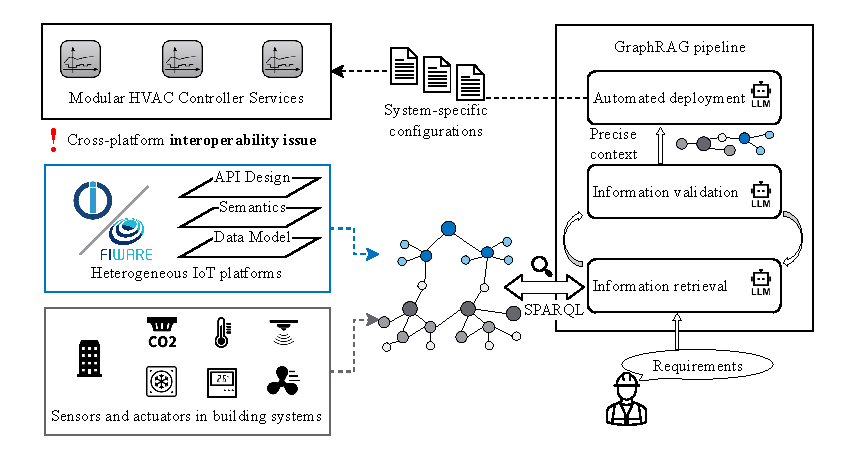
\includegraphics[width=\linewidth]{img/abstract}
    \caption{Overview of the underlying problem and the proposed GraphRAG pipeline}
    \label{fig:abstract}
\end{figure}


% TODO rewrite the paper structure introduction
In the rest of this paper, Section~\ref{sec:related-work} reviews existing literature to contextualize our work, Section~\ref{sec:problem-formulation} specifies the deployment task within the cross-platform environment, Section~\ref{sec:method} details the proposed GraphRAG pipeline, Section~\ref{sec:evaluation} presents the evaluation design and results, Section~\ref{sec:discussion} discusses the findings, and Section~\ref{sec:limitations-conclusion} concludes the paper with limitations and future work.

\section{Related Work}
\label{sec:related-work}
% TODO the main information is not yet defined for related work
\subsection{Building automation and IoT deployment}
Deployment and commissioning are recognised as the labour-intensive part of building system delivery. \citet{crowe2020building} quantify commissioning as a substantial, recurring cost centre and note that controls have grown more sophisticated without the process becoming less manual. \citet{pritoni2021metadata} survey forty metadata schemas and conclude that creating, sustaining, and using semantic models is difficult, labour-intensive, and costly, with semantic gaps blocking cross-building scalability. \citet{fierro2020shepherding} trace the root cause to lifecycle fragmentation: representations produced at design, construction, and operation stages are mutually incompatible, so a usable model must be rebuilt repeatedly. On the platform side, FIWARE provides standard-based, open-source components and an NGSI-LD context model for cross-domain IoT interoperability \citep{bauer2022fiware}. Platforms of the open-source home-automation class, which \citet{setz2021comparison} compare across twenty systems and four in depth, follow a different design philosophy: lightweight, per-instance object trees defined by the operator rather than a shared standard. This strand establishes the pain but treats deployment as an organisational concern. Deployment automation therefore remains a human workflow supported by documentation, spreadsheets, and vendor tooling, and the reviewed literature documents the cost of that workflow more thoroughly than it proposes to reduce it. What it leaves open is a technical method that derives a deployable configuration from the live state of a platform rather than from documentation or human interpretation.

\subsection{Knowledge graphs and ontologies for IoT and buildings}
The semantic-web community supplies the vocabulary layer. Brick \citep{balaji2018brick} defines an ontology and metadata schema for the physical, logical, and virtual assets of a building and their relations, enabling portable applications decoupled from vendor point names. RealEstateCore \citep{hammar2019realestatecore} offers a modular core-plus-extensions ontology for real-estate data that integrates BIM and IoT semantics. The SSN ontology \citep{compton2012ssn} provides the foundational stimulus-sensor-observation model for describing sensors and actuation. These resources are mature and well-governed, and this paper adopts their conceptual distinctions (space, device, point, measurement) as design guidance. The limitation is operational: the community has repeatedly documented that instantiating such a model against a specific building is manual and costly \citep{pritoni2021metadata}, and even automated assistance has targeted sub-problems such as point classification \citep{qian2026brickdicl} rather than full deployment. A second limitation is that ontology classes describe what a point is, not the concrete interface syntax by which a particular platform reads it. The consequence is a persistent gap between a standard that specifies meaning and a platform that specifies syntax, and no reviewed work closes both from live data. What this strand leaves open is the automatic derivation of a usable graph from live, non-standardised platform metadata, and the use of that graph to emit platform-specific configuration.

\subsection{GraphRAG and knowledge-graph-grounded LLMs}
Retrieval-augmented generation (RAG) conditions an LLM on evidence retrieved from an external store \citep{lewis2020retrieval}, which reduces hallucination when the required knowledge sits in self-contained passages.
Engineering metadata rarely has a text form.
Whether a controller can be deployed in a room depends on actuation devices, sensor data points, and how the platform interfaces are available.
The alternative of supplying all metadata in the prompt is unreliable as well, since LLM accuracy drops when relevant information is buried in long inputs \citep{liu2024lost}.
GraphRAG addresses these issues by retrieving over a graph instead of text chunks.
\citet{edge2024local} build an entity graph from a corpus and answer global questions through community summaries, and \citet{peng2025graphragsurvey} organise the field into graph-based indexing, graph-guided retrieval, and graph-enhanced generation, the stages along which the pipeline of this paper is described.

In the building and IoT domain, GraphRAG has so far served mainly as an information-access layer.
LLMs translate natural-language requests into graph queries \citep{iranmaneshLLMassistedGraphRAGInformation2025}, retrieve $k$-hop subgraphs as context for SQL generation in operation and maintenance \citep{liLargeLanguageModelbased2025}, map user intents to action planning in smart homes \citep{jeongOnDeviceIntentReasoning2025}, and answer multi-constraint questions over a graph built from the documentation of an IoT platform \citep{yu2025graphragiot}.
These works show that GraphRAG can bridge the semantic gap between user intent and specific system implementation, but their outputs are answers, queries, or plans, which a human or another system still has to turn into a working configuration.
Their retrieval mechanism also scales poorly with heterogeneous platform data.
With $k$-hop expansion, a small $k$ misses platform-specific interface nodes that lie several relations away from the anchor entity, whereas a large $k$ pulls in neighbourhoods that are irrelevant to the task and inflates the context.

A smaller set of works moves from information access towards automation.
\citet{lyuLLMpoweredAgentOccupantcentric2026} show, without a graph, that enforcing structured LLM outputs is a good practice to enable automated action in building systems.
\citet{peng2026grounding} ground an agentic LLM in a lightweight building semantic layer and automate thermal simulation; the semantic layer, however, relies on specific simplification.
\citet{wenHybridRAGBasedLLMAgents2026} combine keyword, vector, and subgraph retrieval to generate configurations of network optimisation problems.
% TODO these works show automation potential, but they either rely on customised graphs or other information sources.
These works show that automated action is generally feasible via LLMs, but they either rely on customised graphs or other information sources.
A generalized workflow based on comprehensive KGs is still missing.

\subsection{Research questions}
The evaluation addresses two questions.
RQ1: Does GraphRAG enable automated deployment for cross-platform application deployment? % (10 buildings, gemma4:31b)
RQ2: does GraphRAG-based building automation show resilience against increasing data volumes and different model size? (10 to 100, 12b, 26b, 31b)


% TODO is it typical to have such a section?
\section{Problem Formulation and System Overview}
\label{sec:problem-formulation}

\subsection{System overview}
% TODO The FIWARE and ioBroker test environment

\subsection{Task and test buildings}
The task is the demand-based HVAC controller deployment problem of Section~\ref{sec:problem-formulation}.
A deployment case names one target room and one platform and asks for a control strategy and an executable configuration.
The number of rooms in the building is therefore the volume of metadata that has to be searched, not the number of configurations to be produced, which keeps the output of a case constant while the retrieval problem grows.

Test buildings are instantiated on both platforms, FIWARE \citep{bauer2022fiware} and ioBroker.
The ten-room building of E1 is derived from the pilot installations.
The larger instances of E2, at 25, 50, and 100 rooms, are generated by the same instantiation procedure, which preserves the device-to-point topology of the originals and varies sensor availability across rooms, so that strategy selection is not answered by a constant.
Every building is exported twice, once as raw platform metadata and once as a generated knowledge graph, so that the three conditions are supplied with the same building rather than with different data.

Ground truth for a case is an expert-authored pair of a control strategy and a platform configuration.
It is authored from the physical description of the target room and the platform API documentation, independently of the T-box of Figure~\ref{fig:t-box-building-http}, because grading generated output against a schema produced by the same pipeline would be circular.

\section{Method}
\label{sec:method}
We present a GraphRAG pipeline that automates controller deployment in IoT-enabled building systems.
This pipeline follows the three-stage structure of \citet{peng2025graphragsurvey} with use case specific adaptations and enhancements.
Indexing is the graph being built from IoT platform; retrieval is enhanced with a self-reflective validation; generation conditions LLMs on the retrieved subgraph to produce an executable configuration for the controllers.
Each stage is described in the following subsections.

\subsection{Knowledge graph generation from IoT platform}
%A knowledge graph construction pipeline (KGCP) has been proposed in our previous work \citep{duSemiautomatedKnowledgeGraph2026a}, which generates KGs from heterogeneous IoT platforms.
A knowledge graph construction pipeline (KGCP) has been proposed by Du et al. \citep{duSemiautomatedKnowledgeGraph2026a} to generate KGs from heterogeneous IoT platforms, where RDF Mapping Language (RML) documents are semi-automatically defined for specific platforms and used to transform the raw platform metadata into KGs.
This paper reuses the KGCP for the two target platforms, FIWARE and ioBroker.

Besides the existing functions, we further extend the KGCP with a post-processing module to add information about the platform-specific API syntax to the generated KGs by traversing all endpoints nodes and matching them with the corresponding API syntax in the platform specification (swagger or OpenAPI document).

KGs of both platforms are mapped onto the common T-box shown in Figure~\ref{fig:t-box-building-http}, which fixes the vocabulary that the retrieval stage.
\begin{figure*}[ht]
    \centering
    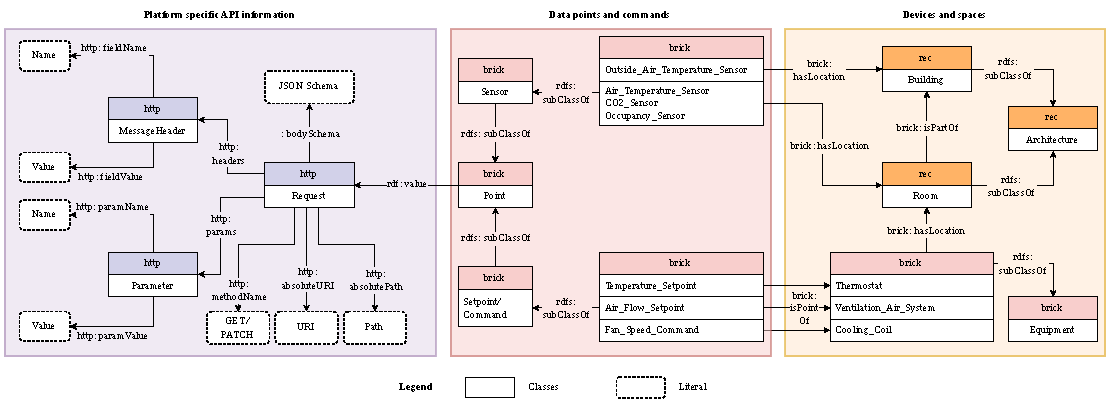
\includegraphics[width=\textwidth]{img/method/T-box-building-http}
    \caption{Common T-box of the generated knowledge graphs, covering devices and spaces, data points and commands, and platform-specific API information. Dashed boxes denote literal values}
    \label{fig:t-box-building-http}
\end{figure*}
It is organised in three blocks, covering devices and spaces, data points and commands, and platform-specific API information.
For the first two blocks, the classes and relations are drawn from Brick \citep{balaji2018brick} and RealEstateCore \citep{hammar2019realestatecore}, which are widely used in building automation domain.
For the third block, the W3C HTTP vocabulary is used to describe the platform-specific API syntax, while the vocabulary is extended with further schema information to describe the structure of the request or response body.

This three-block structure keeps the platform-independent part of a deployment decision separate from the platform-specific one.
The first two blocks state which space contains which device and which quantity each point carries, and they are identical for FIWARE and ioBroker; the third block states how a point is actually read or written, and it is where the two platforms differ.

\subsection{Validation enhanced information retrieval}
Retrieval is performed by generating a SPARQL query rather than by expanding a fixed neighbourhood around an anchor node, as shown in Figure~\ref{fig:graphrag_retrieval_validation_vertical}.
Three inputs enter the SPARQL generation prompt: the KG of the IoT-enabled building, a T-box view obtained by extracting the classes and relations that are actually present in that KG, and a requirement-oriented question.
Extracting the T-box view per graph instead of taking it from the ontology offers the retrieval agent only vocabulary that the queried graph can satisfy.
The prompt further fixes query constraints and rules, which prohibit syntax that bypasses the graph such as \texttt{VALUES}, require optional patterns where data may be absent, scope the context, and constrain the output format.
Since the query is bounded by the task rather than by a hop radius, it reaches the API binding of a data point several relations away from the space without adding the irrelevant neighbourhood that a correspondingly large $k$ would pull in.
\begin{figure}[ht]
    \centering
    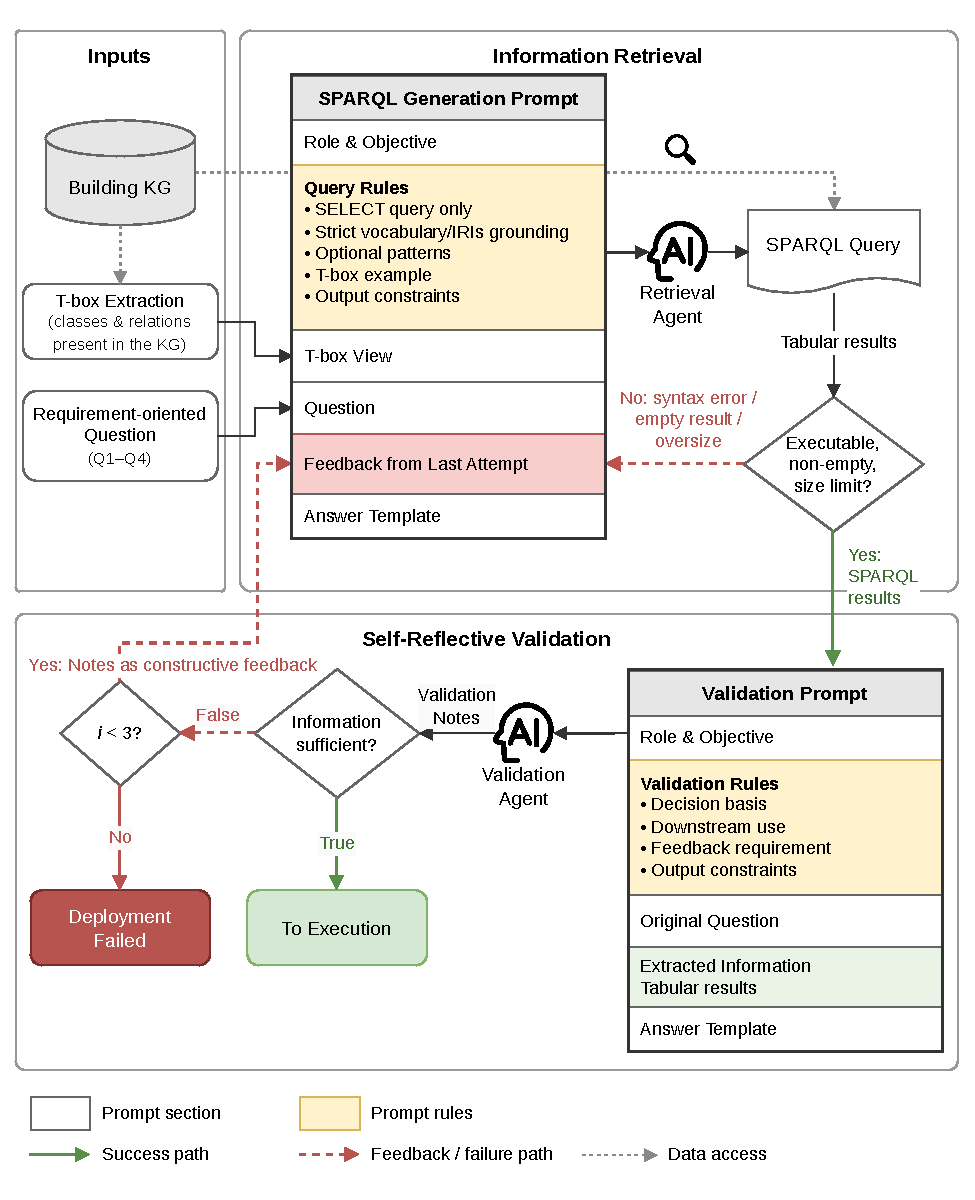
\includegraphics[width=\linewidth]{img/method/graphrag_retrieval_validation_vertical}
    \caption{Prompt structures and workflow of the validation enhanced information retrieval.}
    \label{fig:graphrag_retrieval_validation_vertical}
\end{figure}

As engineering input, a deployment request is decomposed into four requirement-oriented questions, which are answered in a defined order:
\begin{itemize}[noitemsep,topsep=3pt]
\item[Q1] \emph{Space identification}: what rooms can be found?
\item[Q2] \emph{Actuator identification}: which actuators located in, part of, or serving the target room are available for heating, cooling, and ventilation, and which of their data points can be commanded?
\item[Q3] \emph{Sensor identification}: which sensor data points are available in the target room or its shared building environment?
\item[Q4] \emph{API interaction details}: how can each identified actuator data point be written to and each identified sensor data point be read via API calls?
\end{itemize}
The generated query is executed against the KG and accepted only if it is executable, returns a non-empty result, and stays within a size limit; otherwise the failure reason is written back into the next prompt as feedback.

These simple validations ensure that the retrieval agent produces a syntactically valid query that returns a plausibel result, not that the result is sufficient to answer the question.
The retrieved tabular results are therefore passed together with the original question to a validation agent, which judges sufficiency against the downstream use of the information and returns validation notes.
If the information is sufficient, it is handed to the generation stage; if it is not, the notes re-enter the generation prompt as constructive feedback and a further iteration is started, up to three iterations, after which the deployment is reported as failed.
Judging the result against its downstream use is what distinguishes this loop from a single retrieval pass, since a syntactically valid query can still omit, for instance, an important header that is required in an API endpoint.

\subsection{Automated configuration generation}
Each of the four questions is answered with a structured output that follows the answer template of its prompt rather than with free text.
The four answers accumulate into a specification of the deployment case: the target room, the available actuators and sensors, and the API instruction to access those data points.
The executable configuration is produced in a separate deployment prompt that consumes the accumulated answers and the expected format of the structured output.
For all models investigated in this paper, the syntax validity is always given.
The main errors are missing or wrong API information, leading to unsuccessful deployment, or missing data points, leading to a suboptimal strategy being selected.

\section{Evaluation}
\label{sec:evaluation}
The evaluation is organised as two experiments that share one task, one setting of test buildings, and the open-weight models in Gemma4 family.
Experiment E1 fixes the data volume at a ten-room building and the language model at the largest local variant, and compares the three context strategies; it answers RQ1.
Experiment E2 varies the building from ten to one hundred rooms and the model from the 31B variant down to the 12B variant across all three context strategies; it answers RQ2.

Three conditions are defined in Table~\ref{tab:conditions}, which differ only in the context that reaches the generation stage.
B1 supplies the raw platform metadata of the whole building, B2 supplies the generated knowledge graph of the whole building, and P supplies the subgraph retrieved by the validation-enhanced retrieval stage.
All three use the same deployment prompt, the same structured output format, and the same decoding configuration, so that a difference in deployment accuracy can be fairly compared.

\begin{table}[t]
\caption{Evaluation conditions, which differ only in the context supplied to the identical deployment step}
\label{tab:conditions}
\centering\footnotesize
\setlength{\tabcolsep}{4pt}
\begin{tabular}{@{}p{0.6cm}p{2.6cm}p{3.6cm}@{}}
\toprule
ID & Condition & Context supplied \\
\midrule
B1 & Full-context, raw metadata & Platform metadata of the whole building and API specification \\
B2 & Full-context, knowledge graph & Generated KG of the whole building \\
P & GraphRAG (proposed) & Dedicated information retrieved from KG \\
\bottomrule
\end{tabular}
\end{table}

% TODO introduce the metrics
%The primary measure is deployment accuracy, computed element-wise.
%A generated configuration is decomposed into configuration elements, which are the device and point bindings, the parameter values, and the API interaction constructs, and is compared against the ground-truth configuration of the same case: precision is the share of generated elements that match ground truth, recall is the share of ground-truth elements reproduced, and F1 summarises the two.
%The deployment success rate is the share of cases that yield a configuration at all, which separates a wrong configuration from a case in which the retrieval loop reaches its iteration cap or a baseline returns output that does not conform to the required format.
%Strategy correctness is a binary secondary judgement of whether the selected strategy matches the expert strategy.
%
%How a result is reached is measured in two further groups.
%For condition P, the retrieval stage is instrumented per question Q1--Q4 with the number of execution-gate retries, the number of validation iterations, and the size of the retrieved result in rows and in distinct graph nodes.

% TODO introduce the grading process, introduce the datapoints level, and information points level
%Grading is automated.
%Each generated configuration is parsed into a canonical element structure defined per platform and aligned to ground truth by canonical path and semantic role, so that ordering differences inside an order-independent block are equivalent, and values are compared with identifier case and whitespace ignored, platform identifiers canonicalised, and numeric values compared within a fixed tolerance.
%An element that fails canonical alignment counts as unmatched.
%Every cell of the design is run three times with a fixed decoding configuration, and the reported figure is the mean over the repetitions.
%Because each case is solved under every condition and model, the comparisons are paired: accuracy between P and each baseline with paired tests and bootstrap confidence intervals, success rate with the McNemar test, at a Holm-corrected threshold of 0.05.

\subsection{Base case: ten-room building} % TODO change the subsection title
Table~\ref{tab:base} reports E1 on the ten-room building with the 31B variant.
It is read for the gap between P and the two full-context baselines in accuracy, and for the cost at which that gap is obtained, since P issues several retrieval calls where a baseline issues one.
\emph{[PH: statement of the observed gap and its direction, once the runs are exported.]}

% TODO show both datapoints level and information points level.
% TODO dont need to show f1 score
\begin{table}[t]
\caption{Experiment E1, ten-room building, Gemma 4 31B. Deployment accuracy, success rate (SR), prompt tokens and latency per case}
\label{tab:base}
\centering\footnotesize
\setlength{\tabcolsep}{4pt}
\begin{tabular}{@{}p{1.9cm}cccc@{}}
\toprule
Condition & P / R / F1 & SR & kTok & s \\
\midrule
B1 raw metadata & [PH] & [PH] & [PH] & [PH] \\
B2 knowledge graph & [PH] & [PH] & [PH] & [PH] \\
P GraphRAG & [PH] & [PH] & [PH] & [PH] \\
\bottomrule
\end{tabular}
\end{table}

% TODO analyse the results
%  1) Datapoint identification is trivial
%  2) For complete configuration, information point B1 does not work well
%  3) Sorting the information into KG already provides strong support for LLM, boosting the performance, although recall still not reaching 100%
%  4) GraphRAG manages to reach perfect performance.
%  5) Platform specific evaluation?

% TODO figure show case the visited graphs
Figure~\ref{fig:subgraph_visits} makes the retrieval behaviour of a single deployment visible.
For each of the four requirement-oriented questions it shows the part of the building graph that the generated SPARQL query touches, overlaid on the full graph of the ten-room building.
The four subgraphs narrow in sequence, from the rooms of the building in Q1 to the API bindings of the selected data points in Q4, and their union is the context that condition P hands to the deployment step, which is a small fraction of what B2 supplies.

\begin{figure}[t]
\centering
% TODO replace the placeholder box with \includegraphics[width=\linewidth]{img/evaluation/subgraph_visits}
\framebox[\linewidth][c]{\parbox[c][4.2cm][c]{0.92\linewidth}{\centering\emph{[FIGURE PLACEHOLDER: visited subgraph per question Q1--Q4 of one deployment on the ten-room building, overlaid on the full graph]}}}
\caption{Subgraphs visited by the generated queries for Q1--Q4 during one deployment on the ten-room building, shown against the full knowledge graph}
\label{fig:subgraph_visits}
\end{figure}

\subsection{Scaling: building size and model capacity} % TODO change the subsection title
Table~\ref{tab:scaling} reports E2 as a full factorial of the three conditions, the three models, and the four building sizes.

% TODO short models introduction
Three instruction-tuned variants of the Gemma 4 family \citep{gemmaTeam2026gemma4} are used, all served locally through the same runtime and the same decoding settings: the dense 31B variant with 30.7 billion parameters, the mixture-of-experts variant 26B A4B with 25.2 billion total and 3.8 billion active parameters, and the dense 12B variant with 11.95 billion parameters.
All three expose a context window of 256K tokens.

% TODO show the results plot, f1 only, platform-separate or combined?




\subsection{Error analysis} % TODO change the subsection title
% TODO some insight regarding graphRAG method
%   (What is this phenomenon call?) LLM's comprehensive/intelligence could change dramatically, even if only a single ID is changed over the entire prompt. This impact of the ID change is validated through repetition. For example, FIWARE-80-rooms case perform much better than the FIWARE-100-rooms case, with the only difference in prompt being the ID of the target room. Such phenomenon can be observed in all considered models.
%   The SPARQL generation and information retrieval is the most important and critical step in the GraphRAG approach. Almost all error can be attributed to this step.
%   There are some typical errors observed during the development and evaluation: Hallucinated class or property names, Hallucinated wrong target object IRI, SPARQL syntax wrong, Class/Instance misunderstanding

\section{Discussion} % TODO Whether keep this section? Or turn it to subsection like Summary
\label{sec:discussion}
% TODO show it be a summary of the answer to all research questions?


\section{Limitations and Conclusion}
\label{sec:limitations-conclusion}
% TODO real-time ability
The principal limitations are scope and evidence scale. The evaluation covers two platforms and one task family, demand-based HVAC controller deployment; results will not establish the automation of building systems in general, and this boundary is stated so that they are not over-generalised. The graph's quality is bounded by the metadata the platforms expose, so missing or mislabelled points propagate into the graph and the configuration, which the incompleteness arm probes but does not fully resolve. Ground truth depends on expert judgement, and while independence from the graph schema controls the circularity threat, expert variation remains a documented source of uncertainty. Finally, the study is human-supervised: generated configurations are reviewed before application, so any effort saving is measured against a review-inclusive workflow, not a fully autonomous one.

%\subsection{Limitations} TODO check duplication
%Ground truth is authored independently of the T-box, so grading cannot reward the pipeline for reproducing its own encoding.
%The deployment step is identical across the three conditions, so the comparison isolates context assembly rather than generation.
%The buildings beyond ten rooms are generated rather than observed, which controls size and sensor availability but reproduces the topology of two installations only, so the scaling result holds for buildings of that structure.
%The study covers one task family on two platforms with one open-weight model family, and the absence of a proprietary model means that the claim of this paper is about the viability of local models rather than about parity with a larger hosted one.

Within those limits, the paper's finding is that a GraphRAG pipeline over knowledge graphs generated from live IoT platform metadata automates demand-based HVAC controller deployment, outperforming full-context baselines supplied with raw metadata or with the whole graph, and enabling mid-size models to match a larger model. The result supports three contributions: the automatic graph generation method (C1), the retrieval and generation pipeline (C2) as the load-bearing contribution, and the cross-platform evaluation (C3). Two questions remain open: whether graph generation generalises to platforms whose metadata exposes no usable typing, and whether the accuracy advantage persists when the task is raised from a single space to floor or building level, where the retrieved subgraph must span more spaces. The practical implication is that structure supplied by an automatically derived graph can substitute for model scale, which lowers the cost of deploying cross-platform building services on local models.

% =====================================================================
\section*{Data Availability Statement}
The metadata extraction tooling, the knowledge graph generation scripts, the GraphRAG pipeline, and the evaluation harness will be released in a public repository upon publication. Because the cases are derived from building installations, raw platform metadata will be released in a de-identified and, where required, synthetically equivalent form; source code and the evaluation protocol will be openly available without restriction. Ground-truth configurations will be released alongside the de-identified cases.

\section*{AI-Use Disclosure Statement}
AI tools were used in the preparation of this manuscript for research assistance and drafting. Specifically, AI-assisted tooling supported literature discovery and metadata verification for the reference corpus, and AI-assisted drafting was used to produce and revise prose under human direction. All technical design decisions, the task definition, the evaluation protocol, the ground-truth authoring requirements, and the interpretation of the work are the responsibility of the authors. The authors reviewed and edited all AI-assisted content and take full responsibility for the final text.

\section*{Author Contributions (CRediT)}
[Author A]: Conceptualization, Methodology, Software, Writing -- original draft. [Author B]: Investigation, Data curation, Validation, Writing -- review and editing. [Author C]: Supervision, Project administration, Funding acquisition, Writing -- review and editing. [Placeholder author names and roles to be confirmed before submission.]

\section*{Conflict of Interest}
The authors declare no conflict of interest.

\section*{Funding}
This work was supported by [Funder Name] under grant [Grant Number]. [Placeholder: funding details to be confirmed before submission.]

 =====================================================================
\section*{References}
\bibliography{paper}

\end{document}
